\chapter{Multiagent learning}
Until now we have been studying situations in which only one autonomous agent was present in the environment, learning how it could be trained to act in optimal ways. Often, however, there may be multiple agents in the same environment, interacting with each other and learning. This will be the focus of this chapter.

Let us start with two definitions of multiagent systems:

\begin{itemize}
    \item \textit{``Multiagent systems are distributed systems of independent actors called agents that are independently controlled but that interact with one another in the same environment''}. \cite{wooldridge02} \cite{10.1007/978-3-030-01713-2_1}
    \item \textit{``Multiagent systems are systems that include multiple autonomous entities with (possibly) diverging information''}. \cite{ShohamLeytonBrown09}
\end{itemize}

These definitions highlight a few very important characteristics of multiagent systems:

\begin{itemize}
    \item Each agent is \textit{independent} and has its own ``brain'', a (possibly) totally different piece of software controlling the agent.
    \item Agents can take actions in the environment, possibly changing it for the rest of the agents.
    \item Each agent may have a limited -and different, possibly even diverging- view of the environment.
\end{itemize}

Our focus will be the case in which the behavior of the agents is not hardwired, but it can be changed and improved over time towards a goal. Our definition of multiagent learning will then be \textit{``the study of multiagent systems in which one or more of the autonomous entities improves automatically through experience''}.

It is not difficult to imagine how different characteristics of the environment and of the agents might play a role in the overall complexity of the system. As an example, we might consider different scales of environments (such as a city, an ant colony, or a football team) and agents with different degrees of complexity (like a human, a machine, or an insect). A particularly hot topic of research in the field of multiagent systems is cooperation and trust among agents. An agent set in a city, for example, might give less importance to ``behaving well'' compared to one set in a small village, as it tends to interact with different agents each time.

Possibly the most important feature that a system should have to allow agents to learn is \textbf{regularity}. To learn, in fact, we must have something that does not change drastically over time, something that can be relied upon to implement a strategy. We will make the assumption that past experience is somehow predictive of future expectations (dealing with non-stationarity is another topic of current research).

In this chapter we will consider five paradigms:

\begin{itemize}
    \item Online multi-agent reinforcement learning towards an individual utility.
    \item Online multi-agent reinforcement learning towards social welfare.
    \item Co-evolutionary learning.
    \item Swarm intelligence.
    \item Adaptive mechanism design.
\end{itemize}

\section{Online RL towards individual utility}
One of the most studied scenarios in multiagent learning is that in which multiple independent agents take actions in the same environment and learn online to maximize their own utility function.

From a formal point of view (leveraging game theory), this can be considered a \textbf{repeated normal-form game}. It is repeated because it is based on a certain number of repetitions and normal form because it is represented by means of a matrix\footnote{More can be found on Wikipedia: \url{https://en.wikipedia.org/wiki/Repeated_game} \url{https://en.wikipedia.org/wiki/Normal-form_game}}.

\subsection{(Repeated) Normal-form games}
To better understand normal-form games, we introduce the \textit{``Prisoner’s dilemma''}, a standard example of a game analyzed in game theory that shows why two completely rational individuals might not cooperate, even if it appears that it is in their best interests to do so

The game is as such: two members of a criminal gang are arrested and imprisoned. Each prisoner is in solitary confinement with no means of communicating with the other. The prosecutors lack sufficient evidence to convict the pair on the principal charge, but they have enough to convict both on a lesser charge. Simultaneously, the prosecutors offer each prisoner a bargain. Each prisoner is given the opportunity either to betray the other by testifying that the other committed the crime, or to cooperate with the other by remaining silent. The possible outcomes are:

\begin{itemize}
    \item If the two prisoners remain silent (they \textbf{cooperate}), they will both serve one year in prison (corresponding to a payoff of 2).
    \item If A betrays B (A \textbf{defects}), A will be set free (payoff of 3), and B will serve 3 years in prison (payoff of 0).
    \item If the prisoners betray each other, they will both serve two years in prison (with a payoff of 1)\footnote{Adapted from \url{https://en.wikipedia.org/wiki/Prisoner\%27s_dilemma}}.
\end{itemize}

Since it is a normal-form game, we can represent it in a matrix:

\noindent\begin{minipage}{\linewidth}
\centering
\arrayrulecolor{black}
\begin{tabular}{!{\color{black}\vrule}l!{\color{black}\vrule}c!{\color{black}\vrule}c!{\color{black}\vrule}} 
\hline
~         & \multicolumn{1}{l!{\color{black}\vrule}}{Defect} & \multicolumn{1}{l!{\color{black}\vrule}}{Cooperate}  \\ 
\hline
Defect    & (1,1)                                            & (3,0)                                                \\ 
\hline
Cooperate & (0,3)                                            & (2,2)                                                \\
\hline
\end{tabular}
\arrayrulecolor{black}
\end{minipage}

These types of games were initially introduced as one-shot games, where the players knew each other’s reward functions and play the game only once. In this setting, the concept of Nash equilibrium was introduced: a set of actions such that no player has anything to gain from changing their strategy, assuming that the opponent’s strategy is fixed. Games can have one or multiple Nash equilibria. In the case of the prisoner’s dilemma, the only equilibrium is for both agents to defect.

In the case of repeated normal-form games, players interact with one another multiple times, with the objective of maximizing their expected returns over time.

\section{Online RL towards social welfare}
An alternative paradigm to the one just presented is one in which multiple independent agents take actions in the same environment and learn online to maximize a global utility function. These are also called coordination games, where different players coordinate to achieve a given objective (e.g., maximize the global expected return).

An application of this can be seen in the ``Multiagent Cooperation and Competition with Deep Reinforcement Learning'' paper by Tampuu et al. \cite{DBLP:journals/corr/TampuuMKKKAAV15} where two agents learn how to play Pong in a way that maximizes the length of the game, making sure none of the two players lose. To achieve this, the agents learn techniques such as not serving the ball or bouncing it in a straight line, as depicted in the image below.

\begin{figure}
    \centering
    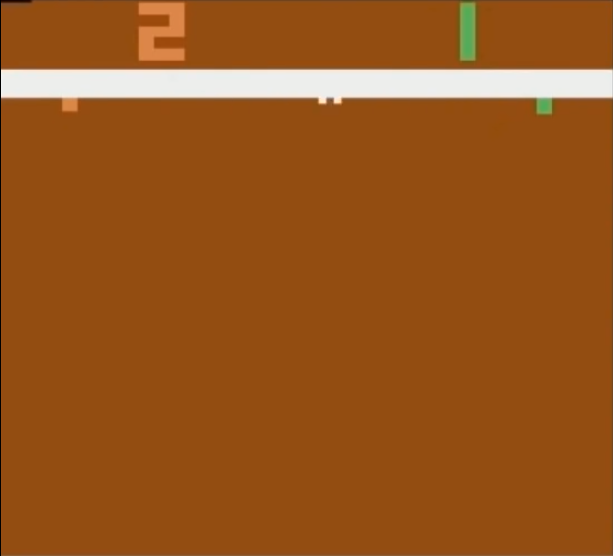
\includegraphics[scale=0.35]{Images/Chapter 9/multiagent-pong.png}
    \caption{Pong being played by two agents}
    \source{Computational Neuroscience Lab at University of Tartu on YouTube}
    \label{fig:ch9-multiagentpong}
\end{figure}

\section{Co-evolutionary approaches}
Evolution can also be used to model and learn agent behavior as well. According to this paradigm, abstract Darwinian models of evolution are applied to refine populations of agents (known as \textit{individuals}) over generations by means of \textbf{evolutionary algorithms}. 

Evolutionary algorithms are made up of five steps\footnote{More can be read on \url{https://towardsdatascience.com/introduction-to-genetic-algorithms-including-example-code-e396e98d8bf3} and \url{https://en.wikipedia.org/wiki/Evolutionary_algorithm}}:

\begin{itemize}
    \item Creation of the initial population by randomly generating agents. Each agent is characterized by a set of parameters called \textbf{genes} (that are joined into strings called \textbf{chromosomes}).
    \item Calculation of the \textbf{fitness score} of the individuals by means of a \textbf{fitness function} (e.g., reward obtained in the episode).
    \item \textbf{Selection} of the best-performing individuals to be used as \textbf{parents} in reproduction.
    \item \textbf{Generation of offspring} by applying \textbf{crossover} and \textbf{mutations} on the parents.
    \item \textbf{Replacement} of the least-fit individuals with new individuals.
\end{itemize}

Repeating the last four steps multiple times allows the refinement of a population. Let us consider the most important parts of evolutionary algorithms more in detail.

\subsection{Fitness function}
The fitness function allows us to evaluate the performance of a certain phenotype (i.e., the actual performance of the behavior of your agent encoded through its genotype). From a more RL-oriented point of view, the fitness function is the equivalent of the performance measure we introduced in \autoref{ch:policygradientmethods}.

\subsection{Selection}
At each generation, we allow the reproduction of only some of the individuals. To choose which of the individuals will reproduce we can adopt two strategies:

\begin{itemize}
    \item Proportionate selection, i.e., the chance of reproducing is proportional to the agent’s fitness with respect to the population’s fitness using the formula:
    \begin{equation*}
        p_i = \frac{fitness_i}{\sum_j fitness_j}
    \end{equation*}
    \item Choosing the top-$K$ individuals of the current generation.
\end{itemize}

\subsection{Cross-over}
Crossover, also called \textit{recombination}, is a genetic operator used to combine the genetic information of two parents to generate new offspring. It is one way to stochastically generate new solutions from an existing population and is analogous to the crossover that happens during sexual reproduction in biology.

\begin{figure}
    \centering
    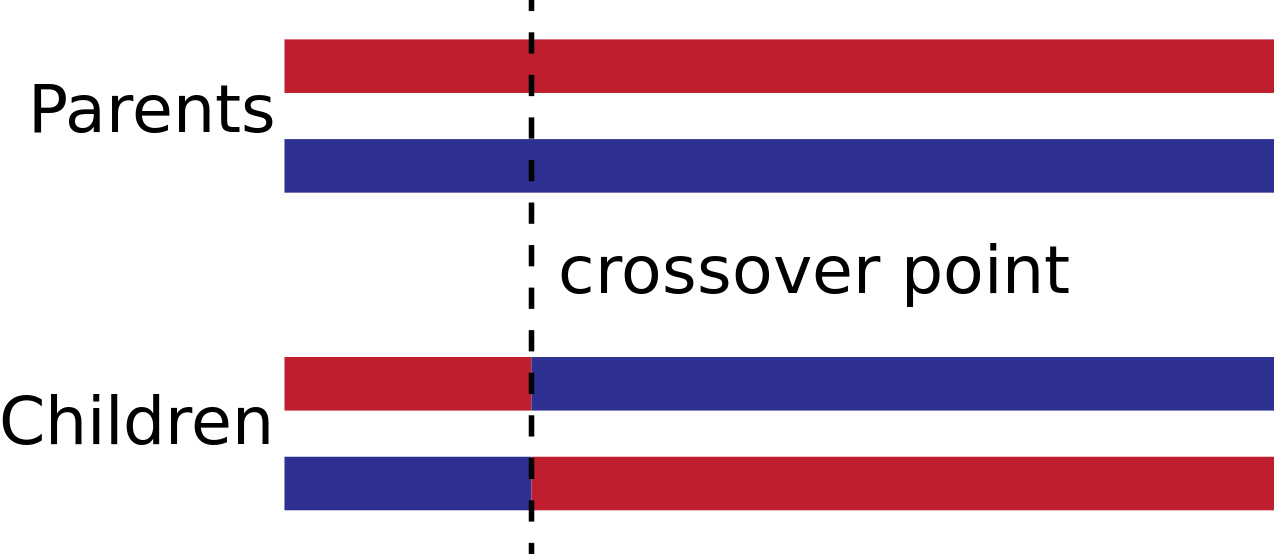
\includegraphics[scale=0.15]{Images/Chapter 9/crossover.png}
    \caption{Crossover in genetic algorithms}
    \source{R0oland on Wikipedia}
    \label{fig:ch9-crossover}
\end{figure}

\subsection{Mutation}
Mutation is a genetic operator used to maintain genetic diversity from one generation of a population of genetic algorithm chromosomes to the next. It alters one or more gene values in a chromosome from its initial state. The classic example of a mutation operator involves a probability that an arbitrary bit in a genetic sequence will be flipped from its original state.

The purpose of mutation in evolutionary algorithms is to introduce diversity into the sampled population. Mutation operators are used in an attempt to avoid local minima by preventing the population of chromosomes from becoming too similar to each other, thus slowing or even stopping convergence to the global optimum.

\subsection{Evaluation and replacement}
At each generation, the fitness of each individual is evaluated, and the population is usually replaced in its entirety by the offspring. Another possible solution is to keep the $n$ ``elite'' individuals from the previous generation to reduce the effects of mutations or sub-optimal fitness evaluation. 

\subsection{Coevolution}
Coevolution is an extension of evolutionary algorithms for domains with multiple agents. By using evolutionary algorithms, we can train a policy to perform a state-to-action mapping. In this approach, rather than update the parameters of a single agent interacting with the environment as it is done in reinforcement learning, one searches through a population of policies that have the highest fittest for the task at hand.